\chapter{Future Work}

Given that SystemNaim was a final year project, and as such we could only put about 9 months of time into it, there are a lot of features that we would have like to have added or expanded upon. This section will go through some higher priority additions that weren't able to be made due to time constraints, but if added would make SystemNaim into a more complete and useful tool.

\section{Actual 'Multi'-FPGA System}

Currently, SystemNaim only allows for two FPGAs to communicate, one parent and one child. Allowing for more FPGAs to be used in tandem would give users the ability to exploit more parallelism within their programs, however it would also come with additional difficulties. The first challenge would be adding an addressing system so that each child FPGA could be identified. It would be likely that the system would just expand, with each child FPGA holding a collection of functions that could be called upon by the parent FPGA when required by the program. The parent FPGA would need to be able to, not only choose the correct function opcode, but also the correct address so that it could call the right off-chip function it required. 

This could be added to the remote modules, which are instantiated on the parent FPGA, with each being designed to store and signal which child FPGA contains their function implementation. The interconnect would then need to tell the channel controller which child FPGA to deliver the opcode and operands to. With SPI this is pretty straightforward, every child FPGA would be connected to the same MISO and MOSI channel and each would have their own SS\_EN (Slave Select Enable) signal, which would be asserted, by the parent FPGA, when that child FPGA was receiving a transaction. In the case of multiple off-chip functions being called at the same time, there would have to be a queue and the parent FPGA would call each function sequentially. Once it had finished calling all the necessary off-chip functions, it would then need to poll each of the activated child FPGAs, until their processing was complete, to return the result.

The polling, in this case, would likely be done in a round-robin fashion. With each child FPGA being sent a polling transaction, as described in \autoref{sec:impl_interconnect}, in order until all results had been returned, an example of this is shown in  \autoref{fig:polling_multi_child}. This does have the potential of causing latency spikes for the entire system. As was explored in \autoref{sec:interconnect}, missing a polling transaction can result in a large amount of additional latency, especially at low SPI Clock speeds, and adding multiple child FPGAs the parent needs to poll can only increase the worst case of a child FPGA missing a polling transaction. The solution for this would be to either know the latency of the off-chip functions, and only poll that child FPGA when it is assumed to have finished computation, or switch to a communication channel where both parties can start a transaction, such as Ethernet.

\begin{figure}[!htb]
    \centering
    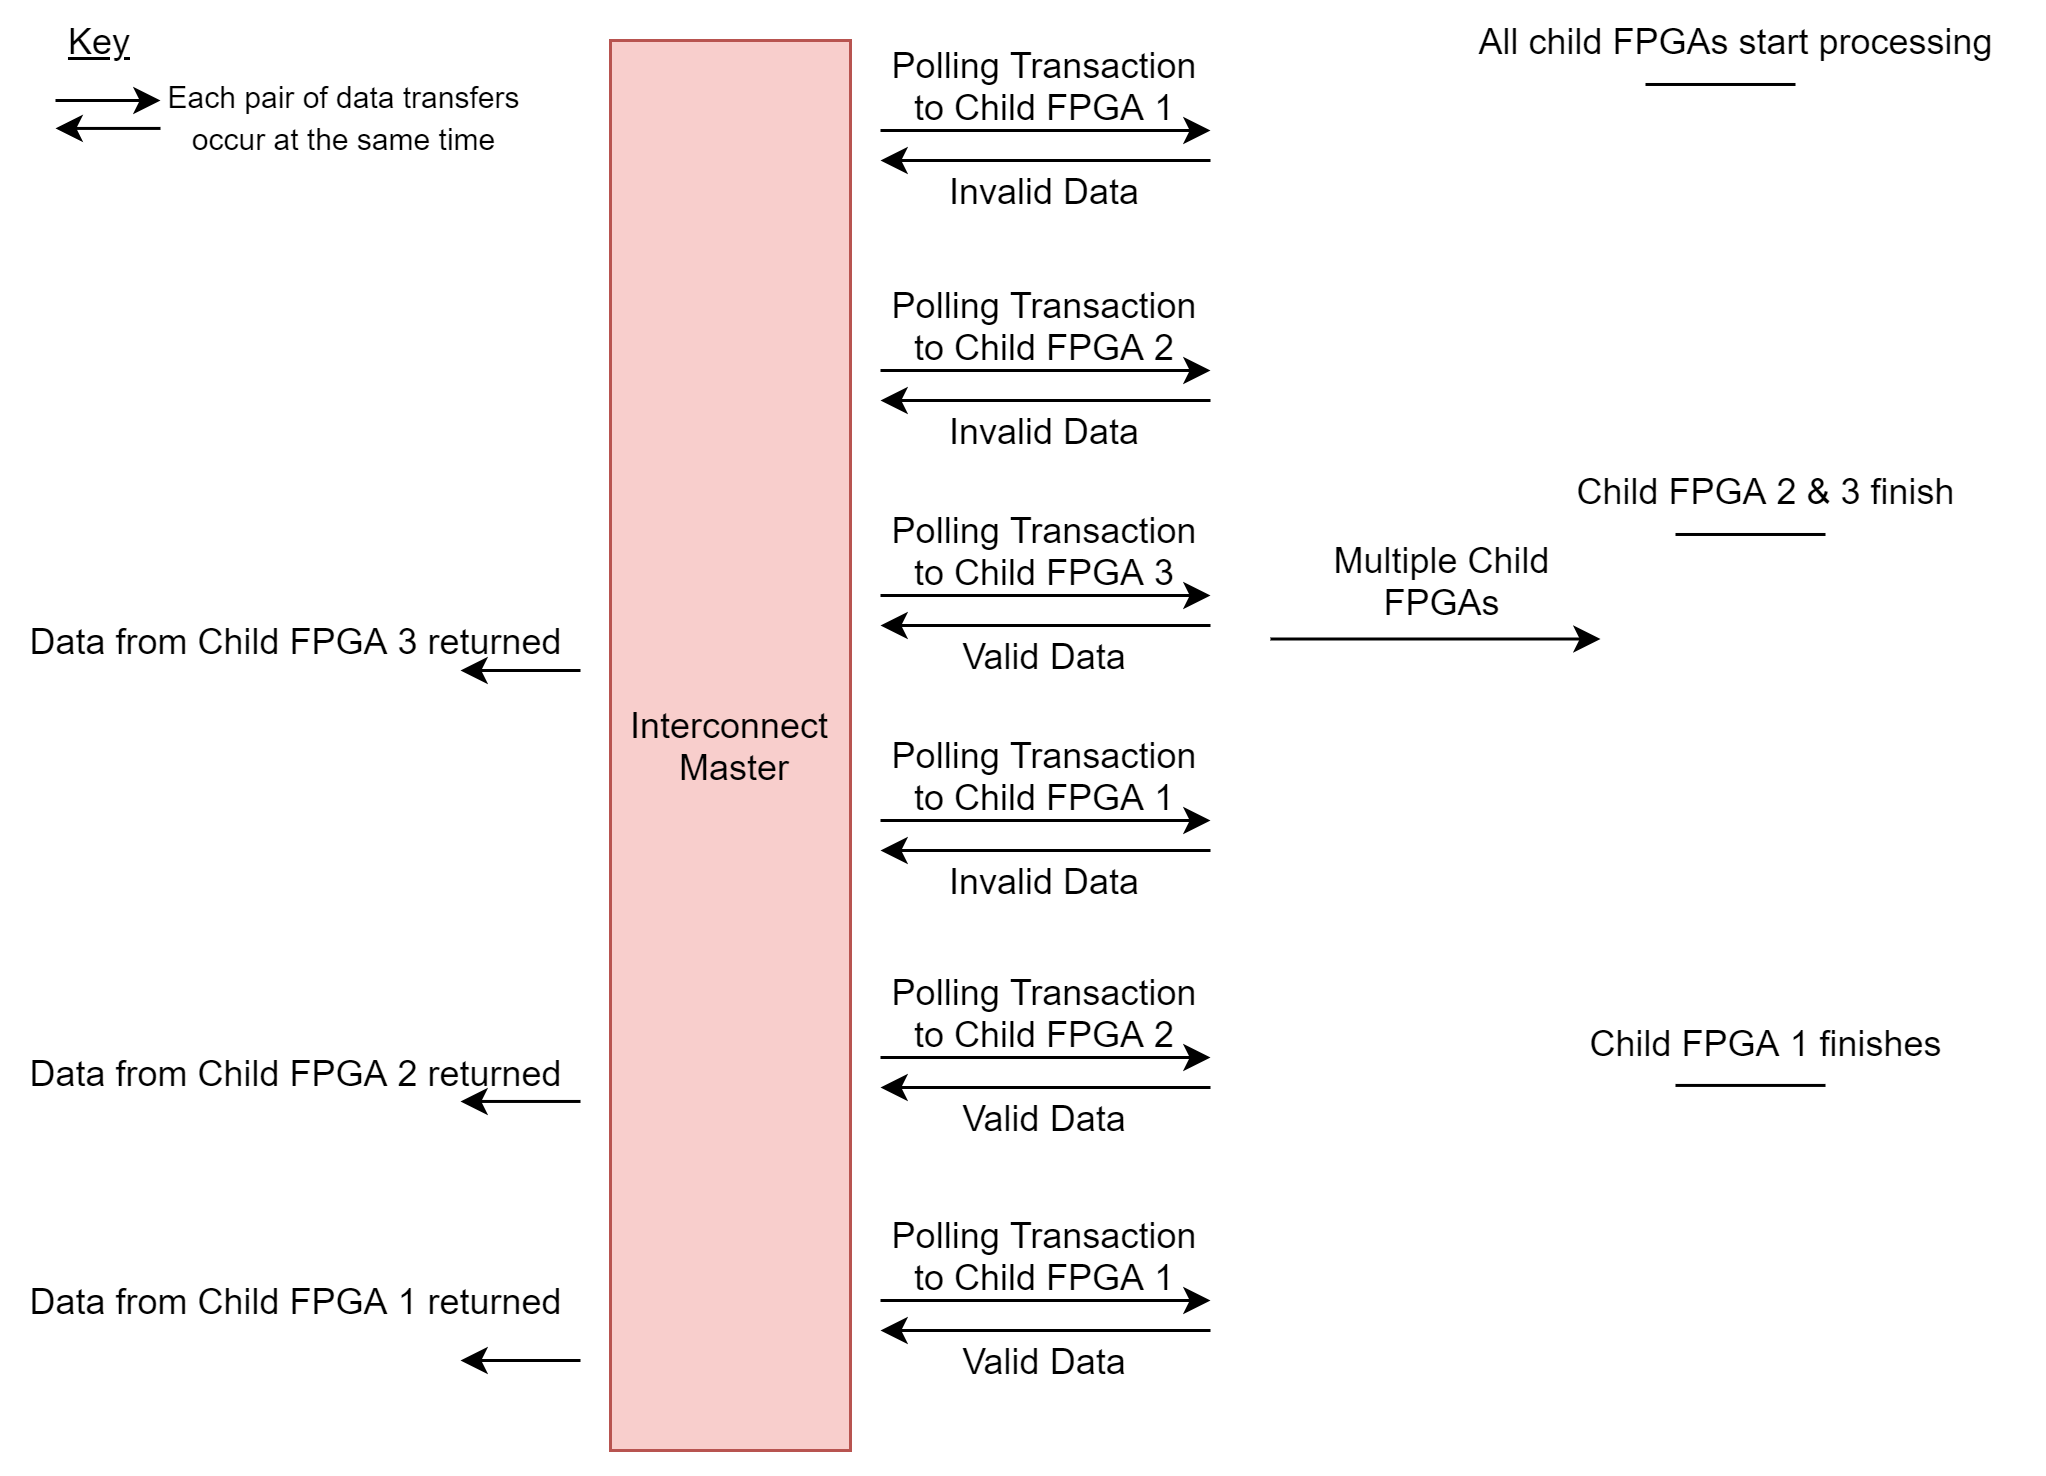
\includegraphics[width=0.9\textwidth]{06_future_work/images/interconnect_polling_multi_child.png}
    \caption{Example of polling transactions with multiple child FPGAs}
    \label{fig:polling_multi_child}
\end{figure}

\subsection{Ethernet}

An Ethernet communication channel would allow child FPGAs to return data to the parent FPGA without the need for constant polling. Furthermore, only one port is required per device, with this never increasing as the system grows larger, and Ethernet can operate at a higher channel bandwidth than SPI thus further reducing the total overhead latency. The downside comes from the added complexity required in SystemNaim's custom hardware. Ethernet requires each device to be identified by a 48-bit number(MAC address) which cannot be assumed to known at runtime, therefore the parent FPGA would initially need to broadcast a request to all child FPGAs, for them to send an Ethernet packet containing their MAC address. As the parent FPGA receives these packets, they would need to store them in a lookup table to be able to communicate, later on in the program, with the child FPGAs.

The additional effort required to get an Ethernet communication channel working would be worth-while as the added channel bandwidth plus capability for larger systems, could allow SystemNaim to implement more latency critical programs as well as, in future, expand the scope to allow computation on the cloud.

\subsection{Changes to the HLS}

When allowing for systems with 3+ FPGAs a decision has to be made as to whether the user should decide which off-chip functions go on which child FPGA. The essence of SystemNaim is to give the user as much control over the end product as possible and merely remove the tedious hardware development aspects, and thus we'd likely incorporate a method that allowed the user to choose which functions are called on which FPGAs. An example of how this is possible is shown in \autoref{fig:multi_fgpa_hls}. Inspiration was drawn from the C++ STL, with the number between the “<>” symbol representing which child FPGA the function would be placed on (0 could mean the function should be run on the parent FPGA). Off all the challenges that would likely be faced when implementing this addition, the modification to the software side is probably the least difficult in a technical sense, however, the final decision on its implementation will define how users interact with this aspect of the system, and thus it is worth conducting a design investigation if there are any plans to ever add this feature in the future.

\begin{figure}[!htb]
    \centering
    \begin{minipage}{0.5\textwidth}
    \begin{minted}{c}
split_fpga{
    holda = <0>hls_test_func_a(h, n);
    holdb = <1>hls_test_func_b(h, n);
    holdc = <2>hls_test_func_c(h, n);
    holdd = <3>hls_test_func_d(h, n);
}
    \end{minted}     
    \end{minipage}
    \caption{Method of allowing user to dictate which child FPGA a function is called on}
    \label{fig:multi_fgpa_hls}
\end{figure}

\section{General HLS Optimizations \& Additions}

As discussed in \autoref{sec:usability} the main downside of SystemNaim is the increase in latency of the hardware it produces, and as explained in DESIGN SECTION the decision to not spend too much time on creating optimal hardware was an intentional one. However, if SystemNaim were to be improved on in the future, optimizing the HDL generated by the HLS would make it much more appealing when compared to creating a dedicated hardware system. Below is a list of different optimizations and additions that could be made to SystemNaim's HLS aspect so that a user could create lower latency or more complex systems.

\subsection{Loop Pipelining}

Pipelining is an example of an optimization that would drastically reduce the latency of any loop-based function. In essence, pipelining allows for multiple iterations of a loop to be computed at the same time and is especially useful when a single iteration may take many cycles. However, in order to implement this feature correctly SystemNaim would need to be able to detect data dependencies both within an iteration and between iterations, and thus an extra step of analysis in the tool would need to be added. 

To illustrate the benefit of loop pipelining, a small example will be looked at. Imagine if we had a loop with 100 iterations and each iteration took 5 cycles. To compute this loop fully would require 500 cycles, with no pipelining. To calculate the latency of this loop with pipelining we need to use the formula found in \autoref{eqn:pipelining}. Initiation interval (II), a term that we haven't used yet, is a defined as the number of cycles between the start of each iteration of the loop. For an unpipelined loop the II is equal to the latency of each iteration. If we were to have an II of 1, the best case, the example loop would only take 104 cycles to compute, thus giving a large reduction in latency. With how prevalent loops are in modern programming, adding this feature would benefit a lot of programs that may be implemented using SystemNaim, but would require an overhaul of the line-to-state model currently in use in order to allow for concurrent hardware.

\begin{equation}
    L_{tot} = L_s + I * (N - 1) \label{eqn:pipelining} 
\end{equation}
where:
\begin{conditions}
L_{tot}    &  is the total latency of the loop \\
I    & is the Initiation Interval(Throughput) \\
N & is the total number of iterations in the loop \\
L_s & is the latency of a single iteration
\end{conditions}


\subsection{FIFO's \& arrays}

In \autoref{sec:dedicated_hardware_computation}, a case when a FIFO would be optimal instead of a loop was given. FIFO's have a lot of uses in hardware design, especially when it comes to acting as the middle man between data-producing and data-consuming hardware modules. They can allow for multiple pipelined loops to act concurrently, without consuming a large amount of resources, and can act as queues for feeding data into a function. Giving access to this hardware construct to users of SystemNaim would allow them to create more complex and optimal systems. This would be the same with arrays, which allow for more complex algorithms to be implemented in SystemNaim. 

Being able to store data is of vital important when creating a modern system, however, when deciding what features SystemNaim needed to implement to prove our aims we realized arrays weren't necessary. Nevertheless, in the future adding both of these constructs would vastly increase the versatility of SystemNaim, but not without their share of challenges. For arrays, multiple sources accessing the same part of memory would require multiplexers so that there wouldn't be any contention, which poses the risk of increasing the latency of each access. In terms of FIFO's, the challenge is more on the HLS side. Giving access to all aspects of the FIFO to the user would be tricky without using a class-based method inspired by C++'s OOP. This would result in potentially too large of a change in syntax, and at that point, instead of making changes to the base C language, it would be worth switching SystemNaim's base language to C++. The additional work while large, could open up more possibilities for different hardware modules to be added in the future, with member functions being the designated way of controlling and interfacing with them.

\subsection{FPGA Pins}

The final addition that we believe SystemNaim would benefit from, is the ability for users to access FPGA pins from their top-level function. Pins on an FPGA are use as I/O and allow for external data streams to be processed on the FPGA. They are essential for most real world FPGA use cases, and giving users the ability to interface with external devices would make SystemNaim a more versatile tool. Users would be able to stream in data from an Ethernet or USB port and user their multi-FPGA system as an accelerator within a larger system. 

Instead of giving access directly to the pins themselves, which would breach the software vs hardware programming paradigm and would defeat the purpose of an HLS tool, we could allow for FIFO's to be implemented at the top-level and then expect the user to develop some hardware to get the data from their external source into said FIFO. This would, of course, require some hardware proficiency on the user's behalf, but it would still give increase the use case of SystemNaim. It would be of interest to actually perform an investigation into the possibility of requiring no hardware proficiency from a user, but still giving them access to I/O pins and ports within the HLS tool.

Another benefit of such a feature would be for child FPGAs to also be able to access their own I/O pins, and thus would be able to consume data from their own sources rather than being given it by the parent FPGA. From \autoref{sec:interconnect}, we know that this would reduce the transfer overhead if we no longer need to send data operands across the channel, therefore, further reducing the latency of the total system.

\section{Inter-FPGA Data Streaming}

The final addition to SystemNaim that will be discusses is changes to the interconnect, specifically, being able to send more than two operands over the channel, and splitting the channel into two channels: control and data.

\subsection{More than 2 Operands}

A limiting factor on the variety of systems SystemNaim can implement is the fact that only two operands can be sent across the communication channel. Many functions require more operands to do any meaningful processing and some may even require an entire, or part of an array. Of course, increasing the number of operands sent over would also cause the transfer overhead, discussed in \autoref{sec:interconnect}, and thus would also increase the latency proportional to the number of integers sent over. 

Currently, the interconnect can only send a fixed number of transactions, and thus if a system required 10 operands for one function call and 3 for another, the function call requiring 3 operands would include 7 wasted transactions. This could be somewhat mitigated by creating a packet system, where a start packet and end packet signal would be sent across the channel to indicate when a transaction begins and when it ends. However, this would introduce an overhead of 2 mandatory transactions, the start and end packets, thus making the latency worse for systems where only few operands are sent over the channel for all off-chip function calls. This would still be a good feature for systems where the range of operands, supplied to off-chip functions, in large, and potentially could be a feature which the user could enable to disable, depending on their needs.

Another issue arises when we consider passing an array to an off-chip function, this array may contain hundreds of integers and in SystemNaim's current implementation, the child FPGA would wait until all the data was sent over the channel before commencing any processing. This would not only take a lot of cycles, especially on low SPI clock speeds, but would also require the storage of all this data. SystemNaim could be modified, however, to allow off-chip functions to start their processing before the entire array is transferred over the channel. This could be done using FIFO's and as long as the off-chip function was only iterating over an array, it would simply be a matter of making the off-chip function poll a FIFO which would be filled up as elements of the array were received by the child FPGA. This would result in the processing of the function and the transmission of data over the channel to happen in parallel, thus decreasing the number of cycles and ridding the need for the child FPGA to store the incoming data. It should be noted that functions with irregular data access patterns would not benefit from this feature, for example, if a loop required elements 1 and 50 from an array to compute the first iteration, then the function would need to wait until element 50 had been transmitted over the channel before starting its processing.

\subsection{Two Channels: Data \& Control}

A feature that would be very useful in system with more than 2 FPGAs would be a split communication channel. The control channel would tell off-chip functions to start processing, while the data channel would feel these function the operands they required. The reason this works well for systems with more than one child FPGA is that the parent FPGA is no longer wasting cycles sending operands over the channel, and can instead send much smaller transactions, thus decreasing the wait time for a child FPGA before it receives its function call. This becomes especially important if SystemNaim allows for more than two operands or even arrays to be sent over, as the second child FPGA to be called on would have to wait for the first child FPGA to receive all of its data, which may take hundreds of channel transactions, before it receives its functions call. 

The data channel in this case could be implemented in many ways. One would be to just have the parent FPGA to only send operands on the data channel, and to do it every time a function call was issued, and example of such a system is shown in \autoref{fig:data_control}. The child FPGA would then just have to wait to receive their operands on this channel, which would be ideal if you had one function call that required many operands and one that required none, as the latter wouldn't need to wait on the data channel and could start it's processing as soon as it received its transaction of the control channel.

However, if you had two function calls, both of which required arrays as input, this system would only marginally reduce the total latency, as the second function would still need to wait for the first to receive all its data. The solution would be separate data channels between the parent FPGA and each child FPGA, as show in \autoref{fig:data_control_ind}. This would take up more pins on the parent FPGA, but it would result in a massive latency drops for systems which were constantly sending large amounts of data between the FPGAs. If this were implemented in tandem with the feature that allows off-chip functions to start processing before all the data has been sent over the channel, SystemNaim would be able to create multi-FPGA systems with small overheads, but which could still exploit parallelism in programs on a larger scale than a single FPGA system would be able to.

\begin{figure}[!htb]
    \centering
    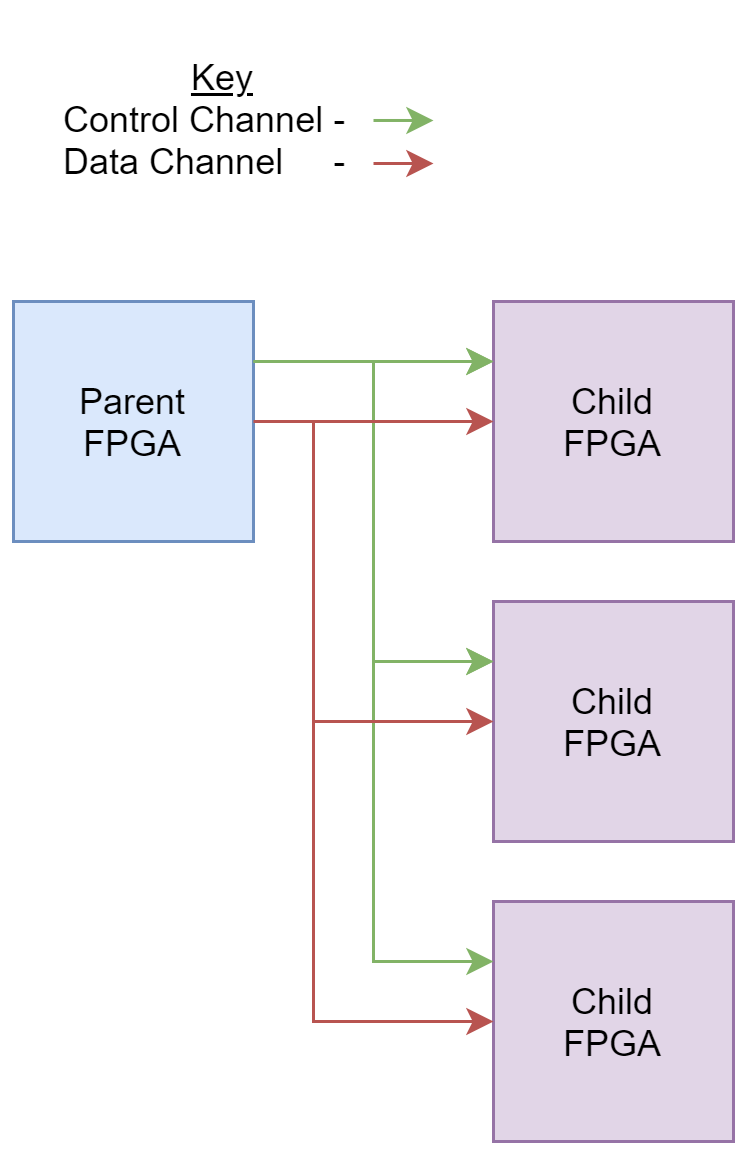
\includegraphics[width=0.4\textwidth]{06_future_work/images/data_control_channels.png}
    \caption{Multi-FPGA system with separate data and control channels}
    \label{fig:data_control}
\end{figure}

\begin{figure}[!htb]
    \centering
    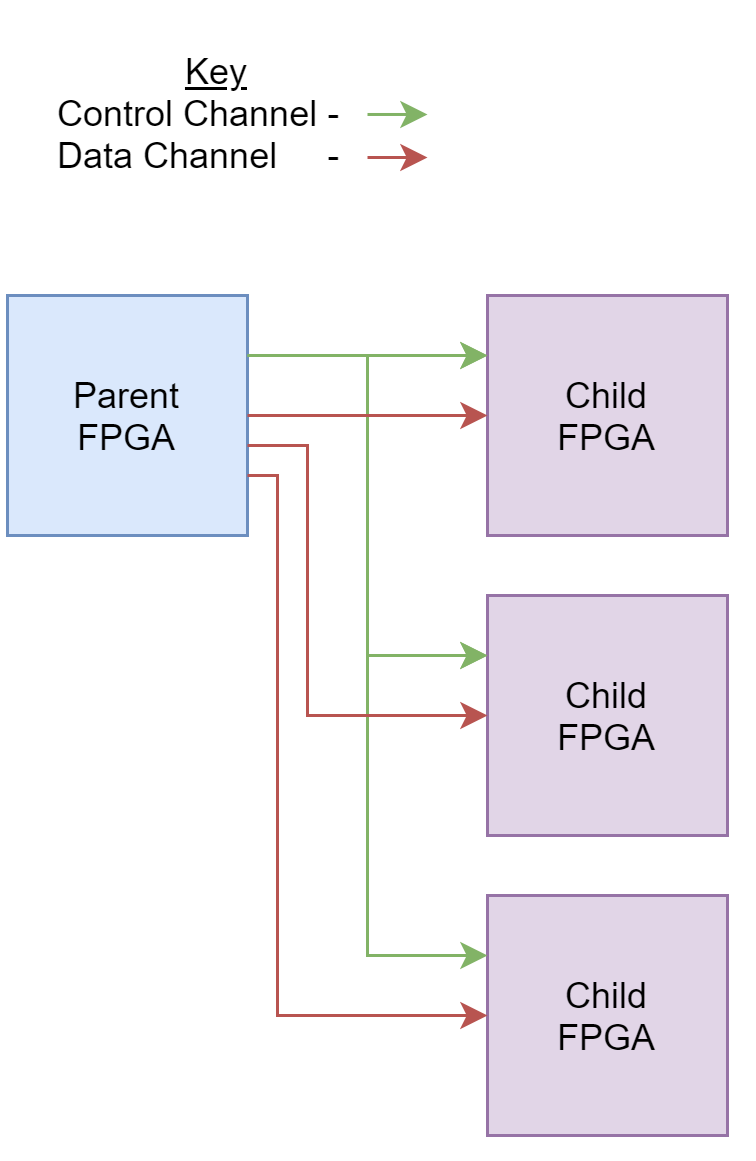
\includegraphics[width=0.4\textwidth]{06_future_work/images/data_control_channels_independent.png}
    \caption{Multi-FPGA system with separate data and control channels. Each child FPGA has their own data channel.}
    \label{fig:data_control_ind}
\end{figure}

\section{Closing Note}

While all the features and solutions above may never be implemented, we feel that exploring and understanding the potential of SystemNaim is important in making the case that it is a stepping stone for future research. We hope that readers of this paper are inspired by these solutions when attempting to create their own multi-FPGA systems, or even their own HLS tool, and can see what possibilities lie ahead for tools such as SystemNaim.